\documentclass[11pt]{article}
\usepackage[margin=1in]{geometry}
\usepackage{volfit_preamble}
\usepackage{tikz}
\usetikzlibrary{arrows.meta,positioning}
\graphicspath{{figures/}}

\title{\textbf{Graph Smile-Extrapolation}\\[2pt]
\large Filling dark nodes from lit neighbours by an OT-regularized Bayesian graph\\[2pt]
\normalsize Vol-Fitter Technical Notes, No.~14}
\author{Vol-Fitter}
\date{\today}

% Note-local notation.
\newcommand{\Kbeta}{K^{\beta}}
\newcommand{\Ldir}{L_{\mathrm{dir}}}
\newcommand{\Lrev}{L_{\mathrm{rev}}}
\newcommand{\Qdel}{Q_{\Delta}}
\newcommand{\Kdel}{K_{\Delta}}
\newcommand{\Arho}{A_{\rho}}

\begin{document}
\maketitle
% Auto-generated by gen_graph.py — do not edit.
\newcommand{\graphdecay}{15}
\newcommand{\graphlitsd}{0.10}
\newcommand{\graphfarsd}{1.52}
\newcommand{\graphsixrows}{%
SPX 1M & dark & 0.641 & 0.11 \\
SPX 3M & lit & 1.000 & 240.09 \\
SPX 6M & dark & 0.641 & 0.11 \\
XLK 3M & lit & 0.550 & 130.07 \\
AAPL 3M & dark & 0.435 & 0.05 \\
MSFT 3M & dark & 0.435 & 0.05 \\
}


\begin{abstract}
This is the Vol-Fitter's headline differentiator: extrapolating sparse smile
observations to a \emph{full universe} of smiles, across expiries and assets, by
propagating signal through a graph whose nodes are smiles $(\text{underlying},T)$.
The mathematics is a Gaussian inverse problem with an optimal-transport-regularized
prior on the \emph{increments}, not the levels --- so the default answer is
``nothing changed from the prior'', and lit calibrations force only the coherent,
graph-plausible changes that explain them. We build the directed graph (a
row-normalized kernel, its stationary distribution, reversible and directed
Laplacians), assemble the increment precision
$\Qdel=D_\kappa+\eta\Ldir^{\beta}+\lambda(\Arho+\nu I)^{-1}$ from three beliefs
(local smallness, directed prediction, low-energy unbalanced-OT flux), prove it is
a proper Gaussian prior, and condition on the lit nodes in covariance form
exploiting $n_{\text{obs}}\ll N$. The production spine --- transported prior,
lit-calibration innovation, graph posterior increment, dark-node reconstruction,
quote comparison --- is described with its provenance hierarchy, data-derived
precision tiers, and per-edge directed amplitude $\beta$. A six-node case file,
solved by the production code, shows the whole mechanism on one page; and a
temporal leave-one-out backtest measures the graph's \emph{skill} over the
transported-prior baseline: on 25 assets across three historical regimes
($\sim$47k held-out scores), neighbour-supported indexes gain $+10$ to $+76$
ATM vol bps and ETFs $+3$ to $+7$; fully-dark single names behind lit
indexes/ETFs --- the product case --- gain $+8$ to $+14$ bps in the
August-2024 spike and $+3.8$ to $+7.2$ fully out-of-sample in the October-2022
bear, with unbiased standardized residuals ($\bar\zeta\approx0$). A case file
documents the harness topology defect that had previously masked the
cross-asset path entirely. A traceability table ties every claim to its module
and test.
\end{abstract}

\tableofcontents
\newpage

%======================================================================
\section{The production problem}
\label{sec:problem}

The desk does not own one smile; it owns a universe of them. A handful of nodes
--- index expiries, a few mega-caps --- are richly quoted (\emph{lit}); the rest
--- single-name expiries, far tenors, the odd weekly that traded twice today ---
are barely quoted or not at all (\emph{dark}). The dark nodes still need
surfaces, and the wrong way to make them is to copy a nearby smile: copying
creates jumps across expiry, ignores cross-asset information, and pretends that
uncertainty did not grow with distance from the data. What production actually
requires is the following.

\begin{invariant}
\begin{enumerate}[leftmargin=1.6em]
\item A dark node stays close to its transported prior unless lit data forces a
move.
\item A move observed at one node propagates only through plausible graph paths:
calendar neighbours first, cross-asset neighbours with smaller trust.
\item Every filled node reports an uncertainty, and uncertainty \emph{widens}
away from the lit observations.
\item The output is a smile-handle vector that retargets into the arbitrage-free
smile machinery of Note~01 --- the graph never emits a raw curve that could carry
butterfly arbitrage.
\end{enumerate}
\end{invariant}

The Vol-Fitter's answer treats the universe as a \emph{graph}: nodes are smiles
$(\text{underlying},T)$, edges encode ``this node informs that one'' (calendar
edges within a name; cross-asset edges from an index or sector ETF to its single
names). A prior surface ties the whole graph together; today's lit calibrations
perturb it; the perturbation propagates.

\begin{heuristic}
The central modelling choice is to regularize the \emph{increment}
$z=x^1-x^0$ --- how each node moved from its transported prior --- rather than
the level $x^1$. The prior already encodes the shape of every smile; what the
graph must infer is only the \emph{change}, and changes are far more coherent
across the graph than levels (an index move drags its names; a calendar shift is
smooth in $T$). Regularizing increments makes ``no change'' the default answer,
and data is required to \emph{earn} every departure from the prior --- exactly
the right inductive bias for a sparsely observed universe.
\end{heuristic}

The carrier is compact: each node propagates its three exact ATM handles
$(\sigma_0,s_0,\kappa_0)$ of Note~01 --- in code \texttt{atm\_vol},
\texttt{skew}, \texttt{curvature} --- as independent Gaussian coordinates (ATM
\emph{vol}, not total variance, so the level coordinate is comparable across
expiries). Reconstruction retargets the posterior handles into an arbitrage-free
smile. For exposition we write one scalar handle per node; production runs the
same construction handle-by-handle with per-handle hyperparameters
(\cref{sec:spine}).

\begin{figure}[H]
\centering
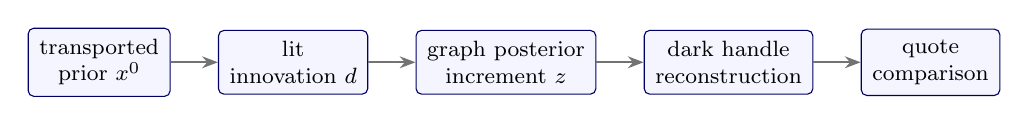
\begin{tikzpicture}[
  box/.style={draw, rounded corners=2pt, align=center, font=\footnotesize,
    minimum height=8mm, inner sep=4pt, fill=blue!4, draw=blue!40!black},
  arr/.style={-{Stealth[length=2mm]}, thick, draw=black!55},
  node distance=6mm,
]
\node[box] (a) {transported\\prior $x^0$};
\node[box, right=of a] (b) {lit\\innovation $d$};
\node[box, right=of b] (c) {graph posterior\\increment $z$};
\node[box, right=of c] (d) {dark handle\\reconstruction};
\node[box, right=of d] (e) {quote\\comparison};
\draw[arr] (a)--(b); \draw[arr] (b)--(c); \draw[arr] (c)--(d); \draw[arr] (d)--(e);
\end{tikzpicture}
\caption{The production spine. The prior is transported first (Note~12). Lit
calibrations produce genuine market innovations
$d=\text{calibrated}-\text{transported}$. The graph posterior spreads those
increments to dark nodes and carries uncertainty into reconstruction, which any
residual dark quotes then score.}
\label{fig:spine}
\end{figure}

%======================================================================
\section{The graph object}
\label{sec:graph}

\begin{assumption}
\label{ass:weights}
The user (or the auto-lattice) supplies raw weights $w_{ij}\ge0$ on the node set
$V=\{1,\dots,N\}$, read ``node $j$ informs node $i$''. Nodes with no
out-neighbours receive a unit self-loop, so every row has positive mass.
\end{assumption}

\begin{definition}[Kernel, stationary mass, conductance]
\label{def:kernel}
Row-normalization gives the row-stochastic kernel
\[
K_{ij}=\frac{w_{ij}}{\sum_\ell w_{i\ell}},\qquad \sum_j K_{ij}=1 .
\]
A stationary distribution is a positive solution of $\pi\T K=\pi\T$,
$\sum_i\pi_i=1$; write $\Pi=\diag(\pi)$. The \emph{reversibilized conductance}
of the unordered pair $\{i,j\}$ is the symmetrized traffic
\[
c_{ij}=\tfrac12\big(\pi_iK_{ij}+\pi_jK_{ji}\big)=c_{ji}\ge0 .
\]
\end{definition}

\begin{remark}[Reducible graphs]
\label{rem:reducible}
Sparse user graphs can be reducible, and then the stationary solve
$(K\T-I)\pi=0$ is singular. Production first attempts the direct dense solve;
only on failure does it fall back to the uniform-teleport (PageRank) damping
$K\mapsto(1-\delta)K+\delta/N$ with $\delta=10^{-3}$, and as a last resort the
uniform mass $1/N$. Irreducible graphs never enter the fallback, so their
$\pi$ is byte-identical to the undamped solve.
\end{remark}

Two symmetric energies are built from these objects, and they answer different
questions.

\begin{definition}[Reversible Laplacian]
\label{def:lrev}
With $B\in\R^{N\times E}$ the signed incidence matrix of the conductance edges
and $C=\diag(c_e)$,
\[
\Lrev=BCB\T,\qquad
z\T\Lrev z=\tfrac12\sum_{i,j}c_{ij}(z_i-z_j)^2 .
\]
$\Lrev$ measures undirected \emph{roughness}: it is PSD and annihilates
constants. It never enters the prior directly; its role is to supply the
geometry of the transport term (\cref{def:mobility}).
\end{definition}

\begin{definition}[$\beta$-weighted directed residual]
\label{def:ldir}
For a per-edge amplitude matrix $\beta$ (with $\beta_{ii}=1$), let
$\Kbeta_{ij}=K_{ij}\beta_{ij}$ (the Hadamard rescaling $K\!\circ\!B$). The
\emph{directed residual energy} of an increment field $z$ is
\[
\mathcal E_{\mathrm{dir}}(z)
=\norm[\Big]{\big(I-\Kbeta\big)z}_{\Pi}^2
=z\T\Ldir^{\beta}z,
\qquad
\Ldir^{\beta}=(I-\Kbeta)\T\,\Pi\,(I-\Kbeta).
\]
\end{definition}

The directed residual is the \emph{prediction} rule: node $i$ is compared with
the $K$-weighted, $\beta$-scaled forecast $\sum_jK_{ij}\beta_{ij}z_j$ made by
its in-neighbours, and the disagreement is charged at the node's stationary
importance $\pi_i$. The kernel decides \emph{who} predicts ($K$ = trust); beta
decides \emph{how large} the transported increment should be along that edge
($\beta$ = amplitude). A one-vol-point index ATM move may imply a
$0.7$-vol-point move in a single name while the skew handle translates at a
different rate --- so $\beta$ is per-edge, per-direction and per-handle, and
$\beta_{ij}\neq\beta_{ji}$ is allowed. Setting $\beta\equiv1$ recovers the plain
directed rule exactly (byte-identical, test-locked).

\begin{proposition}[Directed residuals are safe Gaussian penalties]
\label{prop:dir-psd}
For every real amplitude matrix $\beta$ and every $\pi$ with $\pi_i>0$,
$\Ldir^{\beta}$ is symmetric positive semidefinite.
\end{proposition}

\begin{proof}
$\Ldir^{\beta}=R\T\Pi R$ with $R=I-\Kbeta$ is a Gram matrix in the
$\Pi$-weighted inner product: for every $z$,
$z\T\Ldir^{\beta}z=\sum_i\pi_i\big(z_i-\sum_jK_{ij}\beta_{ij}z_j\big)^2\ge0$,
and symmetry is manifest from the factorization.
\end{proof}

\begin{remark}
Unlike $\Lrev$, the directed residual does \emph{not} annihilate constants
unless every row of $\Kbeta$ sums to one: with $\beta\equiv1$ a constant field
is a perfect prediction ($\Ldir\1=0$), but an amplifying edge
($\beta>1$) makes even a constant move partially ``unexplained''. That is
intentional --- amplitude is a statement about how moves scale, not a
reparametrization of trust.
\end{remark}

The stationary solve and the two-line directed Laplacian are exactly the
production computation (\cref{app:ref} verifies the distilled listing against
\texttt{volfit.graph} to $10^{-12}$):

\begin{lstlisting}[caption={The stationary distribution and the
$\beta$-weighted directed residual (distilled from
\texttt{graph/\{build,beta\}.py}).},label={lst:graph}]
def stationary(K):                # solve pi^T K = pi^T, sum(pi) = 1
    n = len(K); S = K.T - np.eye(n); S[-1] = 1.0  # last row = mass constraint
    rhs = np.zeros(n); rhs[-1] = 1.0
    return np.linalg.solve(S, rhs)

def directed_laplacian_beta(K, pi, B):   # L_dir^beta, PSD for ANY B (Prop 1)
    M = np.eye(len(K)) - K * B           # Hadamard rescale: trust x amplitude
    return M.T @ (pi[:, None] * M)
\end{lstlisting}

%======================================================================
\section{The increment prior}
\label{sec:prior}

The increment field receives the Gaussian prior
$z\sim\mathcal N(0,\Kdel)$, $\Kdel=\Qdel^{-1}$, with precision
\begin{equation}
\boxed{\;\Qdel=D_\kappa+\eta\,\Ldir^{\beta}+\lambda\,(\Arho+\nu I)^{-1}.\;}
\label{eq:Qdelta}
\end{equation}
The three terms are three distinct answers to ``what is a plausible change?''

\begin{description}[leftmargin=1.7em,style=nextline]
\item[Local smallness, $D_\kappa=\diag(\kappa)$, $\kappa_i>0$.]
A dark, poorly connected node must not invent a large move on its own. This is
the cost of moving alone, and it is what makes the prior proper
(\cref{prop:proper}).
\item[Directed prediction, $\eta\,\Ldir^{\beta}$.]
A node's move should be explained by the nodes that inform it --- the calendar
and cross-asset propagation rule of \cref{def:ldir}.
\item[Transport tangent norm, $\lambda\,(\Arho+\nu I)^{-1}$.]
A move is also plausible when it could have been \emph{produced} by a coherent,
low-energy flux along the edges, with net creation and destruction (sources and
sinks) priced by $\nu$. This is the tangent norm of unbalanced optimal transport
on the graph \cite{Chizat2018,Peyre2019}, and it asks a genuinely different
question from $\Ldir$: not ``do my neighbours predict me?'' but ``could this
pattern of changes have flowed here cheaply?''
\end{description}

\begin{definition}[Mobility Laplacian]
\label{def:mobility}
For a positive reference density $\rho$ on the nodes (default: the stationary
mass), the \emph{mobility} of edge $e=\{i,j\}$ is
$m_e=c_e\,\theta(\rho_i,\rho_j)$ with $\theta$ the logarithmic mean
$\theta(a,b)=(a-b)/(\log a-\log b)$ \cite{Maas2011}, and
\[
\Arho=B\,\diag(m_e)\,B\T .
\]
$\Arho$ is PSD and annihilates constants; it is $\Lrev$ with conductances
reweighted by how much probability mass is locally available to move.
\end{definition}

The transport term is easiest to read through its dual.

\begin{proposition}[Screened-potential form of the OT term]
\label{prop:ot-dual}
For $\Arho\succeq0$ symmetric and $\nu>0$,
\[
z\T(\Arho+\nu I)^{-1}z
=\sup_{\phi\in\R^N}\Big\{2\inner{z,\phi}-\phi\T(\Arho+\nu I)\phi\Big\},
\]
and the maximizer is the solution of the screened Poisson equation
$(\Arho+\nu I)\phi=z$.
\end{proposition}

\begin{proof}
The map $\phi\mapsto2\inner{z,\phi}-\phi\T(\Arho+\nu I)\phi$ is strictly concave
because $\Arho+\nu I\succ0$; its stationarity condition is
$(\Arho+\nu I)\phi=z$, and substituting the maximizer
$\phi^\star=(\Arho+\nu I)^{-1}z$ gives the stated value.
\end{proof}

So a graph increment is cheap under the third term exactly when the screened
potential needed to explain it is small: smooth, transportable patterns need a
gentle potential; an isolated spike at a badly connected node needs a large one.
The allowance $\nu$ prices the sources --- as $\nu$ grows, un-transported
creation becomes cheaper and the term relaxes toward a scaled identity.

\begin{proposition}[The increment prior is proper]
\label{prop:proper}
Assume $\kappa_i>0$ for all $i$, $\eta\ge0$, $\lambda\ge0$, $\nu>0$, and
$\Arho\succeq0$ symmetric. Then $\Qdel$ in \eqref{eq:Qdelta} is symmetric
positive definite, hence $z\sim\mathcal N(0,\Qdel^{-1})$ is a proper Gaussian
law.
\end{proposition}

\begin{proof}
$D_\kappa\succ0$. $\Ldir^{\beta}\succeq0$ by \cref{prop:dir-psd}. Since
$\Arho\succeq0$ and $\nu>0$, $\Arho+\nu I\succ0$, and the inverse of a
positive definite matrix is positive definite. A nonnegative combination of PSD
matrices added to the positive definite $D_\kappa$ is positive definite;
symmetry is preserved by each term (production additionally symmetrizes
$\tfrac12(Q+Q\T)$ against floating-point drift).
\end{proof}

\begin{heuristic}
The prior is a three-person committee. The first member says ``do not move
unless you must'' ($\kappa$). The second says ``if you move, the nodes that
inform you should have predicted it'' ($\eta$). The third says ``and the whole
pattern of moves should have been transportable along the graph without an
implausibly expensive flow'' ($\lambda,\nu$). In the shipped default the third
member abstains ($\lambda=0$): the machinery is implemented, tested and exposed
in the UI (``$\lambda$ OT flux (0 = off)''), but the default product
configuration runs the classical $D_\kappa+\eta\Ldir$ regime until the selected
universe has enough topology for transportability to say something trust-worthy.
\end{heuristic}

%======================================================================
\section{Conditioning on the lit nodes}
\label{sec:posterior}

Let $S=\{s_1,\dots,s_m\}$ be the lit nodes, $H_S:\R^N\to\R^m$ the selector of
their coordinates, and $d_S=x^1_S-x^0_S$ the observed innovations with
per-node observation precisions $r_s>0$:
\[
d_S=H_Sz+\epsilon,\qquad \epsilon\sim\mathcal N\big(0,R^{-1}\big),\quad
R=\diag(r_s).
\]
The baseline $x^0$ itself carries finite precision $p^0_i>0$ (the provenance
tiers of \cref{sec:spine}), which folds into the predictive covariance:
\[
\mu^-=0\ (\text{or a drift}),\qquad
K^-=\Kdel+P_0^{-1},\qquad P_0=\diag(p^0).
\]
Infinite trust in the baseline is the limit $P_0^{-1}\to0$.

\begin{proposition}[Covariance-form graph update]
\label{prop:cov-update}
The posterior law of $z$ given $d_S$ is Gaussian with
\begin{align}
S_y&=H_SK^-H_S\T+R^{-1}, \label{eq:sy}\\
\alpha&=S_y^{-1}\big(d_S-H_S\mu^-\big), \label{eq:alpha}\\
\mu^+&=\mu^-+K^-H_S\T\,\alpha, \label{eq:mup}\\
K^+&=K^--K^-H_S\T\,S_y^{-1}\,H_SK^-. \label{eq:kp}
\end{align}
\end{proposition}

\begin{proof}
The joint law of $(z,d_S)$ is Gaussian with covariance
\[
\begin{pmatrix}K^- & K^-H_S\T\\ H_SK^- & H_SK^-H_S\T+R^{-1}\end{pmatrix},
\]
and \eqref{eq:sy}--\eqref{eq:kp} is the Schur-complement conditioning of the
first block on the second \cite{RasmussenWilliams2006}.
\end{proof}

\begin{remark}[Why covariance form]
Production uses \eqref{eq:sy}--\eqref{eq:kp} rather than a posterior-precision
assembly because $m=n_{\text{obs}}\ll N$: only the $m$ observed \emph{columns}
$K^-H_S\T$ and one $m\times m$ solve are needed, and the reported marginals
$K^+_{ii}$ come from a single \texttt{einsum} over those columns --- no dense
$N\times N$ posterior matrix is ever formed. A posterior variance
$\le0$ (numerically broken input) raises immediately rather than propagating a
negative band.
\end{remark}

\begin{caution}
The confidence reported for node $i$ is $\pi^+_i=1/K^+_{ii}$ --- the reciprocal
of the \emph{marginal} posterior variance --- and never $(Q^+)_{ii}$, the
diagonal of the posterior precision. The two differ whenever nodes are
correlated (always): $Q^+_{ii}$ answers the conditional question ``how pinned is
$i$ with all other nodes \emph{held fixed}?'', which overstates confidence
precisely at the dark nodes whose neighbours are themselves uncertain. The
accessor is \texttt{GraphPosterior.marginal\_precision}, and the credible bands
of \cref{fig:prop} use the marginal variance.
\end{caution}

\Cref{fig:prop} is a real run of the production solver on a calendar chain with
one lit node: the unit innovation propagates outward and decays, the far node
receiving only \graphdecay\% of the lit move while the posterior standard
deviation grows from \graphlitsd\ at the lit node to \graphfarsd\ at the far end
--- the credible band widening exactly as invariant~3 demands. \Cref{fig:eta}
shows the directed-smoothness weight $\eta$ controlling the reach.

\begin{figure}[H]
\centering
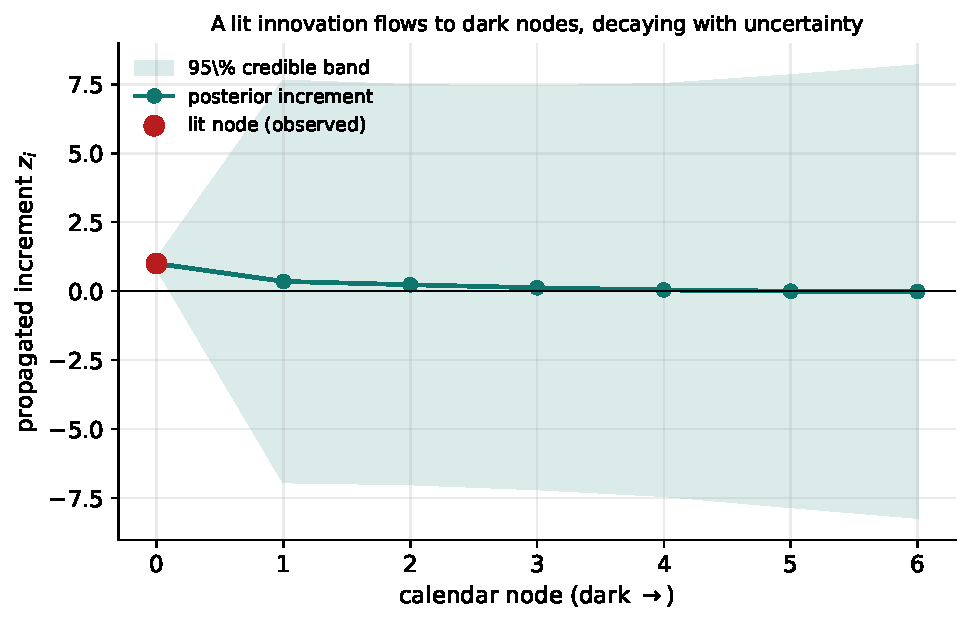
\includegraphics[width=0.98\textwidth]{fig_graph_prop.pdf}
\caption{A one-handle innovation observed at the lit 3M node (red) propagates
along a calendar chain and decays. The same update widens the uncertainty: the
far node inherits \graphdecay\% of the lit move while the posterior standard
deviation grows from \graphlitsd\ to \graphfarsd. Panel B is the reason the
caution above exists: what is plotted is the \emph{marginal} band width,
which honestly decays away from the data.}
\label{fig:prop}
\end{figure}

\begin{figure}[H]
\centering
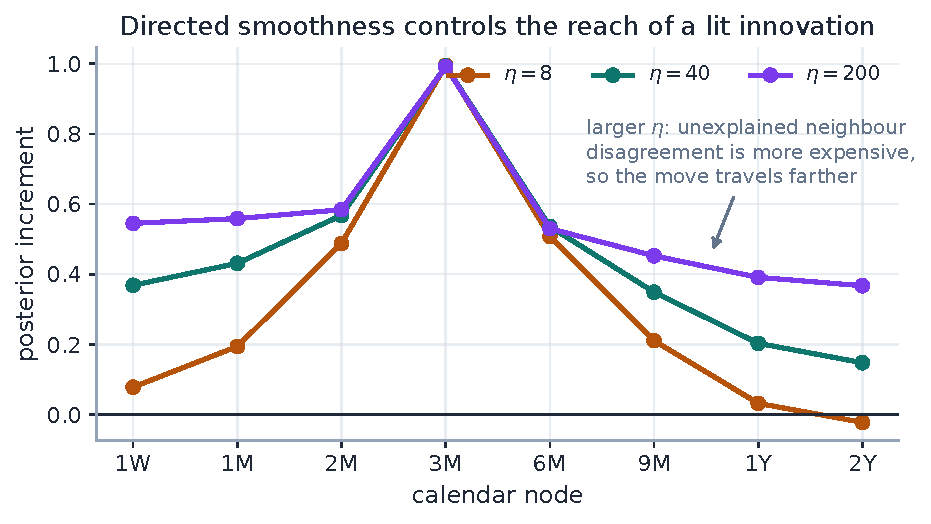
\includegraphics[width=0.9\textwidth]{fig_graph_eta.pdf}
\caption{The directed-smoothness weight $\eta$ controls reach. Small $\eta$
leaves the move local (the $\kappa$ member of the committee wins); large $\eta$
makes unexplained neighbour disagreement expensive, so the move travels
farther along the chain.}
\label{fig:eta}
\end{figure}

%======================================================================
\section{The production spine}
\label{sec:spine}

\subsection{Transported prior and provenance}

Each node's baseline $x^0$ is the prior's three handles \emph{transported to the
current spot} (Note~12). The prior is resolved by a strict hierarchy, each level
carrying its provenance tag and a validity flag: \texttt{active\_transported}
(a saved prior) $\to$ \texttt{nearest\_expiry\_transported} (precision scale
$0.25$) $\to$ \texttt{today\_bootstrap} ($0.05$; not valid for validation ---
scoring against it would be circular) $\to$ \texttt{flat\_atm} ($0.01$;
diagnostic only). The provenance sets the baseline precision tier: a fragile
fallback must never impersonate a saved prior.

\subsection{Data-derived precision, not hand-set weights}

Both precisions entering \cref{prop:cov-update} are \emph{derived}:
\[
r_s=\mathrm{clip}\!\Big(\tfrac{1}{\max(\mathrm{rms},\,\mathrm{floor})^2}
\cdot f_{\text{quotes}}\cdot f_{\text{spread}}\cdot f_{\text{age}}\cdot
c_h,\ \cdot\Big),
\qquad
p^0_i=\mathrm{clip}\!\Big(\mathrm{SOURCE}\cdot f_{\text{age}}\cdot
f_{\text{transport}}\cdot c_h,\ \cdot\Big),
\]
with $c_h=$ \texttt{HANDLE\_CONFIDENCE} $=[1,1,0.01]$ (curvature is far harder
to identify than level or skew) and per-handle floors and caps so that no
single calibration dominates and no baseline vanishes. At the design point
(active prior, dense fresh quotes, tight spread) the tiers reproduce the legacy
regime $[10^6,10^6,10^4]$ exactly.

\subsection{Lit innovation, not manual shift}

For each lit node the observation is $d=\text{calibrated handles}-
\text{transported prior handles}$: the node is actually fitted, in pure-market
mode, so the innovation is the genuine market-versus-prior move and not itself
prior-anchored. Dark nodes are never observations --- a dark quote may be used
\emph{afterwards} for validation, never during propagation.

\subsection{Per-handle hyperparameters}

Production solves \eqref{eq:Qdelta} once per handle with a per-handle regime
$(s_h,\eta_h)$: $\kappa=\texttt{kappaScale}/s_h^2$,
$\eta=\eta_h\cdot\texttt{etaScale}$,
$\lambda=\texttt{lambdaScale}/s_h^2$, where $s_h$ is the handle's natural move
scale ($0.03$ vol for ATM, $0.05$ for skew, $0.5$ for curvature) and $\eta_h$
its base coupling ($2\!\times\!10^4$, $7\!\times\!10^3$, $70$). Scaling by
$1/s_h^2$ keeps the \emph{dimensionless} strength of each belief comparable
across handles.

\subsection{Amplitude: where $\beta$ comes from}

In the production API, $\beta$ comes from the per-edge editor and the
\texttt{crossBeta} scalar, entering only $\Ldir^{\beta}$ (never the mobility
term). The temporal backtest harness additionally builds \emph{vol-normalized}
betas --- $\beta_{\text{abs}}=\beta_{\text{vn}}\cdot\sigma_{\text{from}}/
\sigma_{\text{to}}$ with $\beta_{\text{vn}}=\sqrt{T_{\text{to}}/T_{\text{from}}}$
on calendar edges and $0.7/0.8/0.6$ for index/ETF/same-sector-name edges,
capped at $3$ --- so that ``a one-vol move over there'' is translated into local
vol units before amplitude is applied. That construction lives in the backtest
edge builder; the core solver just consumes whatever $\beta$ it is given.

\subsection{Reconstruction and comparison}

The posterior handles at a dark node are retargeted (Note~01's ATM-orthogonal
chart, $w_0=\sigma_0^2\tau$) into an exact arbitrage-free LQD slice --- shape
modes untouched, invariant~4 by construction. If the app is displaying SVI or
Multi-Core SIV, the parametric family is refitted to the reconstructed target so
the overlay matches the displayed model; for local volatility the reconstruction
becomes the projection target of an affine LV calibration. The credible band
rides along from the level handle's marginal variance. Where a dark node does
own a few quotes, the reconstruction is scored against them --- weighted RMS,
inside-spread hit rate, and the standardized residual
$\zeta=(\text{actual}-\text{posterior mean})/\sqrt{\text{posterior variance}}$
--- an honest, never-trained-on measure.

%======================================================================
\section{A six-node case file}
\label{sec:case}

\begin{example}[title={Case file: one index move, five listeners}]
\textbf{Setup.} The miniature universe of \cref{fig:six-node}: an SPX calendar
chain (1M/3M/6M), the sector ETF XLK~3M, and two technology names AAPL/MSFT~3M.
Calendar edges carry high trust both ways; XLK listens to SPX far more than SPX
listens back; the names listen to their sector ETF first and the broad index
second, with weak feedback edges keeping the chain irreducible. Lit nodes: SPX~3M
calibrates $+1.00$ handle units above its transported prior, XLK~3M $+0.55$.
The single names carry weaker baseline precision, so they are \emph{allowed} to
listen more.

\textbf{Mechanism.} The SPX calendar neighbours inherit most of the index move
through the high-conductance calendar edges. AAPL and MSFT inherit a blend of
the XLK and SPX innovations through their cross-asset edges, shrunk toward zero
by $\kappa$ and their own baselines. Precision is highest at the lit nodes and
decays along every path (solved by the production
\texttt{build\_graph}/\texttt{build\_increment\_prior}/\texttt{posterior\_update};
the table is generated, not typed):

\begin{center}
\begin{tabular}{llrr}
\toprule
Node & Role & Posterior increment & Marginal precision\\
\midrule
\graphsixrows
\bottomrule
\end{tabular}
\end{center}

\textbf{Lesson.} The graph does not fill dark nodes by nearest-neighbour
copying. Every dark node receives a \emph{shrinkage forecast with a provenance
path and a confidence}, and the confidence is what lets downstream quote
comparison distinguish ``the reconstruction is wrong'' from ``the reconstruction
is far from lit information''.
\end{example}

\begin{figure}[H]
\centering
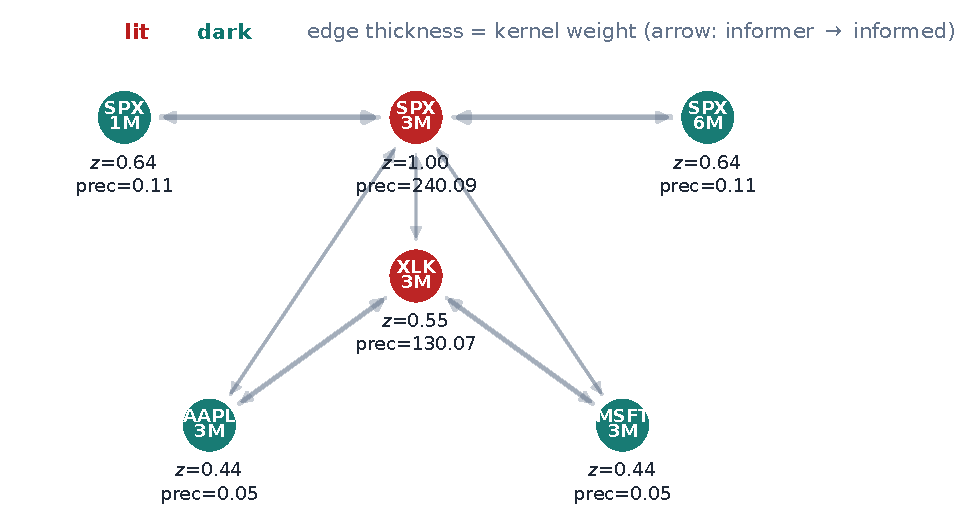
\includegraphics[width=0.88\textwidth]{fig_graph_sixnode.pdf}
\caption{The six-node case file, solved by the production code. Red nodes are
lit innovations; teal nodes are dark posterior reconstructions, each labelled
with its posterior increment $z$ and marginal precision. Arrow direction is
informer $\to$ informed; thickness is the kernel weight after row
normalization.}
\label{fig:six-node}
\end{figure}

%======================================================================
\section{Does it work? The leave-one-out backtest}
\label{sec:backtest}

The graph's value is its \emph{skill} over the transported-prior baseline: does
propagating the lit innovations beat just keeping the (transported) prior? The
temporal leave-one-out harness answers exactly that. Per consecutive captured
day pair, freeze day-$(T{-}1)$ as the prior, transport it under the
spot-dynamics regime $R$ (Note~12), form the lit innovations, propagate, and
compare the graph posterior at \emph{held-out} nodes with their actual day-$T$
calibration --- against the pure transported-prior baseline. Because the
transport regime itself is uncertain, the harness brackets it: $R=0$
(sticky-moneyness) leaves an underperformer's baseline unmoved and
\emph{over}-credits the graph; $R=1$ (sticky-strike) bakes in the full leverage
effect and \emph{under}-credits it. The truth lies between.

On the spike regime (August 2024; 18 consecutive day pairs, 4134 scored
held-out node evaluations):

\begin{itemize}[leftmargin=1.4em]
\item \textbf{Fill a sparse node from its lit neighbours} (withhold each clean
node): the graph \emph{decisively} beats transport --- ATM skill $+37.1$ vol bps
at $R=0$ and $+25.6$ at $R=1$, wing RMS skill $+6.6$ and $+2.6$ bps, with
standardized residuals unbiased ($\bar\zeta=-0.01$) and slightly conservative
($\operatorname{std}\zeta=0.90$ and $0.72$) --- the bands are, if anything, a
touch too wide, which is the safe side of miscalibration. The driver is the
calendar coupling.
\item \textbf{Cross-asset to fully-dark names} (lit = index/ETF only): skill
$\approx0$ on this pilot. Two explanations were recorded at the time --- a
pinning baseline precision (a $96$ bp SPX innovation was measured to move a
fully-dark AAPL node by $0.01$ bp) and a structurally starved 8-asset universe.
\emph{Both later proved to be symptoms of a harness topology defect}, not
properties of the method or the data; the case file below documents the
defect, its fix, and the corrected verdict.
\end{itemize}

\begin{figure}[H]
\centering
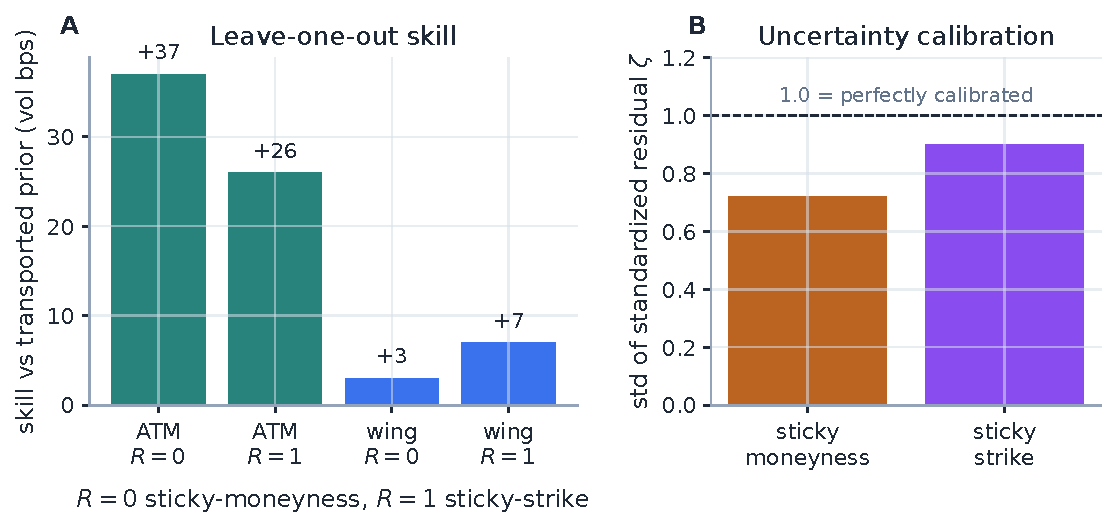
\includegraphics[width=0.95\textwidth]{fig_graph_backtest.pdf}
\caption{The leave-one-out verdict (8-asset pilot run; the 25-asset benchmark
below ships as a regenerable HTML artifact). Left: skill over the transported
prior for the neighbour-supported use case, bracketed by the two transport
regimes --- the graph adds $+25.6$ to $+37.1$ ATM vol bps. Right: the
standardized-residual std is below one in both regimes: the posterior bands are
slightly conservative, never overconfident.}
\label{fig:backtest}
\end{figure}

\subsection{Case file: the transient-name topology defect}
\label{sec:loo-casefile}

The pilot's cross-asset null survived the move to the full 25-asset capture
(3 regimes $\times$ 19 day pairs, $\sim$47k held-out scores): the liquid-split
design returned ATM skill $+0.000$ in \emph{every} regime --- graph RMS equal
to the baseline to three decimals --- even though same-sector name--name and
index$\to$name edges were live. Exact zeros are not damping; they are
disconnection, and the diagnosis found it in the \emph{harness}, not the
solver. The backtest edge builder emitted cross-asset edges one-way (informer
$\to$ name; indexes and ETFs received calendar edges only). Under the trust
kernel $K$ of \cref{def:kernel} the single names were therefore
\emph{transient} states of the directed walk: all their mass drains into the
index/ETF calendar chains and none returns, so the stationary distribution
puts $\pi_i=0$ on every name, the reversibilized conductance
$c_{ij}=f(\pi,K)$ vanishes on every edge touching a name, and the increment
prior decouples the dark names entirely. No signal ever arrived: the dark
baseline precision never mattered (measured post-fix: a dead lever ---
identical posteriors at $0.25\times$, $0.05\times$ and $0.01\times$ the tier),
and the ``$0.01$ bp'' pilot measurement was this artifact. The production
auto-lattice is unaffected: its cross-ticker edges are symmetric, so
$\pi>0$ everywhere.

The fix (\nolinkurl{EdgeConfig.cross_reverse_frac}, default $1$) emits the
reverse edge --- the name informs its index/ETF informer --- with the
\emph{inverse} amplitude $\beta$, so both directions encode the same linear
relation and no second economic claim is introduced; names become recurrent
and their conductance is nonzero. Setting the fraction to $0$ reproduces the
legacy disconnected topology (test-locked).

\subsection{The 25-asset verdict on fully-dark names}
\label{sec:loo-25}

With the topology fixed, the liquid-split design was re-run over all three
regimes at reach $\eta=10$ and cross-conductance $\times25$ --- tuned on the
spike regime only, so October 2022 and July 2023 are out-of-sample for the
knob choice. Dark single names only ($\sim$3.4--3.7k scores per regime and
transport regime $R$; ATM, bps):

\begin{center}\small
\begin{tabular}{@{}lccccc@{}}
\toprule
regime & $R$ & graph RMS & baseline RMS & skill & $\zeta$ (mean/std)\\
\midrule
spike Aug-2024 & 0 & 489.5 & 503.7 & $+14.2$ & $-0.01$ / $1.10$\\
spike Aug-2024 & 1 & 475.5 & 483.5 & $+7.9$  & $-0.06$ / $1.02$\\
high Oct-2022  & 0 & 193.6 & 200.9 & $+7.2$  & $-0.02$ / $0.78$\\
high Oct-2022  & 1 & 174.3 & 178.1 & $+3.8$  & $-0.03$ / $0.70$\\
low Jul-2023   & 0 & 451.6 & 452.3 & $+0.7$  & $-0.04$ / $1.91$\\
low Jul-2023   & 1 & 452.0 & 452.8 & $+0.8$  & $-0.06$ / $1.85$\\
\bottomrule
\end{tabular}
\end{center}

Three conclusions. \textbf{(i)} Cross-asset extrapolation to fully-dark names
carries real, quotable skill in stressed regimes: $+7.9$ to $+14.2$ bps in the
spike and $+3.8$ to $+7.2$ fully out-of-sample in the October-2022 bear, with
unbiased, honest-to-conservative bands. \textbf{(ii)} In the calm regime the
skill is $\approx0$ --- never negative --- because single-name moves there are
earnings-idiosyncratic and carry no systematic component the graph could
transport; the mechanism cannot manufacture idiosyncratic information, only
carry shared repricing. \textbf{(iii)} The one dishonest cell in the pack is
the calm regime's dark-name bands ($\operatorname{std}\zeta\approx1.9$,
overconfident): the dark posterior uncertainty should widen when a name's own
regime is idiosyncratic (an event/earnings-aware term in the dark baseline
precision) --- an open follow-up.

%======================================================================
\section{What is original here}
\label{sec:original}

The ingredients are classical --- Gaussian conditioning, graph Laplacians,
stationary Markov chains, unbalanced-OT tangent norms. The synthesis for
volatility is specific:
\begin{enumerate}[leftmargin=1.6em]
\item \textbf{Increments, not levels} \eqref{eq:Qdelta}: ``no change from the
transported prior'' is the default dark-node answer, and lit data must earn
departures.
\item \textbf{Three beliefs in one precision}: local smallness, directed
prediction and transportable flux are separately tunable in a single proper
Gaussian prior (\cref{prop:proper}).
\item \textbf{Trust and amplitude separated}: $K$ chooses the neighbours,
$\beta$ scales their increments, per edge, per direction and per handle
(\cref{prop:dir-psd} keeps every choice safe).
\item \textbf{Smile handles as the carrier}: the propagated coordinates are the
exact ATM handles of Note~01, so every reconstruction retargets into an
arbitrage-free smile rather than a free-floating scalar field.
\item \textbf{Skill, honestly measured}: the leave-one-out harness scores
against the transported prior --- the strongest cheap competitor --- bracketed
by the two stickiness regimes, with calibrated standardized residuals, rather
than against a straw-man flat fill.
\end{enumerate}
To our knowledge, propagating arbitrage-free smile handles through an
OT-regularized Bayesian graph to reconstruct an unquoted universe is novel.

%======================================================================
\section{Traceability}
\label{sec:traceability}

\begingroup
\small
\setlength{\tabcolsep}{3pt}
\begin{longtable}{@{}p{0.27\textwidth}p{0.16\textwidth}p{0.28\textwidth}p{0.25\textwidth}@{}}
\caption{Claims in this note and the code/tests that lock them.}\\
\toprule
Claim & Object & Code anchor & Test anchor\\
\midrule
\endfirsthead
\toprule Claim & Object & Code anchor & Test anchor\\ \midrule
\endhead
Kernel, $\pi$, conductance; teleport fallback only when reducible &
\cref{def:kernel,rem:reducible} &
\nolinkurl{volfit/graph/build.py} &
\nolinkurl{test_graph_example.py}\\
Operators PSD, annihilate constants &
\cref{def:lrev,def:mobility} &
\nolinkurl{volfit/graph/operators.py} &
\nolinkurl{test_graph_example.py::test_operators_are_psd_and_annihilate_constants}\\
$\beta$-residual PSD for any $\beta$; $\beta\equiv1$ byte-identical &
\cref{prop:dir-psd} &
\nolinkurl{volfit/graph/beta.py} &
\nolinkurl{test_graph_beta.py}\\
Increment precision matches \eqref{eq:Qdelta}; proper prior &
\cref{prop:proper} &
\nolinkurl{volfit/graph/prior.py} &
\nolinkurl{test_graph_example.py::test_increment_precision_matches_note}\\
Covariance-form update; innovation system &
\cref{prop:cov-update} &
\nolinkurl{volfit/graph/posterior.py} &
\nolinkurl{test_graph_example.py::test_innovation_system_matches_note}\\
Reported confidence is marginal, $1/K^+_{ii}$ &
\cref{sec:posterior} &
\nolinkurl{GraphPosterior.marginal_precision} &
\nolinkurl{test_graph_example.py::test_posterior_table_matches_note}\\
OT term implemented; pulls toward baseline &
\cref{prop:ot-dual} &
\nolinkurl{volfit/graph/operators.py}, \nolinkurl{prior.py} &
\nolinkurl{test_graph_example.py::test_ot_weight_pulls_toward_baseline}\\
Provenance / precision tiers &
\cref{sec:spine} &
\nolinkurl{volfit/graph/precision.py}, \nolinkurl{api/graph_nodes.py} &
\nolinkurl{test_graph_precision.py}, \nolinkurl{test_graph_node_priors.py}\\
Lit innovation $=$ calibrated $-$ prior &
\cref{sec:spine} &
\nolinkurl{api/graph_extrapolation.py} &
\nolinkurl{test_graph_extrapolate_solve.py}\\
Reconstruction is arbitrage-free &
invariant~4 &
\nolinkurl{api/graph_reconstruct.py} &
\nolinkurl{test_graph_reconstruct.py}, \nolinkurl{test_graph_lv.py}\\
Held-out nodes predicted, not pinned &
\cref{sec:backtest} &
\nolinkurl{api/graph_backtest.py} &
\nolinkurl{test_graph_backtest.py}\\
Directed vol-normalized backtest edges &
\cref{sec:spine} &
\nolinkurl{backend/backtest/graph_edges.py} &
\nolinkurl{test_graph_loo_backtest.py}\\
Reverse cross edge keeps names recurrent ($\pi>0$); fraction $0$ = legacy
disconnected topology &
\cref{sec:loo-casefile} &
\nolinkurl{EdgeConfig.cross_reverse_frac} &
\nolinkurl{test_graph_loo_backtest.py::test_index_to_name_direction_and_vol_normalization}\\
\bottomrule
\end{longtable}
\endgroup

\appendix
%======================================================================
\section{Hyperparameter atlas}
\label{app:atlas}

\begin{longtable}{p{0.26\textwidth}p{0.16\textwidth}p{0.50\textwidth}}
\caption{Graph-extrapolation hyperparameters.}\label{tab:atlas}\\
\toprule Knob & Default & Role\\ \midrule
\endfirsthead \toprule Knob & Default & Role\\ \midrule \endhead
\multicolumn{3}{l}{\emph{Surfaced}}\\ \midrule
\texttt{graphKappaScale} & $1.0$ & Scales the local precision
$\kappa=\texttt{kappaScale}/s_h^2$; larger keeps nodes closer to the prior.\\
\texttt{graphEtaScale} & $1.0$ & Scales the directed-prediction weight
$\eta=\eta_h\cdot\texttt{etaScale}$ (autotunable, \cref{app:perf}).\\
\texttt{graphLambdaScale} & $0.0$ & OT tangent-norm weight (off by default;
``$\lambda$ OT flux'').\\
\texttt{graphNu} $\nu$ & $0.1$ & Source/sink allowance in the screened operator
$\Arho+\nu I$.\\
\texttt{crossBeta} / \texttt{edgeBetas} & $1.0$ / --- & Per-edge directed
increment amplitude (\cref{def:ldir}).\\
graph \texttt{calendarWeight} / \texttt{crossWeight} & $10.0$ / $2.0$ &
Auto-lattice edge trusts (calendar vs cross-ticker). \emph{Not} the LQD
calendar-slack penalty of Note~10, which shares the name
\texttt{calendarWeight} in \texttt{OptionsSettings}.\\
\texttt{flatAtm} & \texttt{false} & Allow the flat-ATM diagnostic baseline.\\
\midrule
\multicolumn{3}{l}{\emph{Hidden}}\\ \midrule
\texttt{GRAPH\_PRIOR\_HYPER} & $(s_h,\eta_h)$ & Per-handle scale and base
coupling: $(0.03,2{\cdot}10^4)$ ATM, $(0.05,7{\cdot}10^3)$ skew, $(0.5,70)$
curvature.\\
\texttt{HANDLE\_CONFIDENCE} & $[1,1,0.01]$ & Per-handle relative confidence
(curvature is weakly identified).\\
\texttt{SOURCE\_BASE} & tiered & Provenance precision: active
$10^6\gg$ nearest $2.5{\cdot}10^5\gg$ bootstrap $5{\cdot}10^4\gg$ flat
$10^4$.\\
\texttt{OBS/BASE\_PRECISION} floors/caps & per-handle & No single fit dominates;
no baseline vanishes.\\
\texttt{STATIONARY\_DAMPING} & $10^{-3}$ & Teleport damping, reducible graphs
only (\cref{rem:reducible}).\\
\texttt{sink\_self\_loop} & $1.0$ & Self-loop weight for out-degree-zero rows.\\
\bottomrule
\end{longtable}

%======================================================================
\section{Performance notes}
\label{app:perf}

\begin{enumerate}[leftmargin=1.6em]
\item \textbf{Covariance-form conditioning.} Only the $n_{\text{obs}}$ observed
columns of $K^-$ and one $n_{\text{obs}}\times n_{\text{obs}}$ solve are
formed; the marginal variances come from one \texttt{einsum} over those columns.
Cheap whenever few nodes are lit --- the production case.
\item \textbf{Dense at $O(10^3)$.} $\Qdel$ and $\Kdel=\Qdel^{-1}$ are formed
densely, fine up to $\sim10^3$ selected nodes. The deferred Phase-10 sparse path
replaces the two dense $N\times N$ inverses with sparse solves
$(\Arho+\nu I)u=v$ and a Hutchinson diagonal estimator for universes
$\gg10^3$.
\item \textbf{$\beta\equiv1$ golden.} The per-edge beta machinery is
byte-identical to the plain directed rule at $\beta=1$ (test-locked), so it is
strictly additive.
\item \textbf{$\eta$ autotune.} \texttt{POST /graph/autotune} chooses
\texttt{etaScale} by leave-one-out cross-validation over the seven-point grid
$\{0.1,0.25,0.5,1,2,4,10\}$ --- the $O(7\,n_{\text{obs}}N^3)$ cost the sparse
path targets.
\end{enumerate}

%======================================================================
\section{Reference implementation}
\label{app:ref}

The prior and the posterior update are each a handful of lines. The listing
reproduces the production \texttt{build\_increment\_prior} and
\texttt{posterior\_update} (with $\lambda=0$) to better than $10^{-10}$ on the
six-node case file of \cref{sec:case}, including the marginal precisions
printed in the table.

\begin{lstlisting}[caption={Increment prior and covariance-form update
(distilled from \texttt{graph/\{prior,posterior\}.py}).}]
def increment_prior(K, pi, kappa, eta, B=None):
    B = np.ones_like(K) if B is None else B
    L = directed_laplacian_beta(K, pi, B)
    Q = np.diag(np.full(len(K), kappa)) + eta * L
    return np.linalg.inv(0.5 * (Q + Q.T))   # K_Delta

def posterior(K_delta, base_prec, obs, y, r):
    k_minus = K_delta + np.diag(1.0 / base_prec)  # + P0^{-1}
    cols = k_minus[:, obs]             # observed columns only
    S_y = cols[obs, :] + np.diag(1.0 / r)  # H K^- H^T + R^{-1}
    alpha = np.linalg.solve(S_y, y)        # innovation weights
    mean = cols @ alpha                    # mu^+  (mu^- = 0)
    var = np.diag(k_minus) - np.einsum(    # marginal K^+_{ii}:
        "ij,ji->i", cols, np.linalg.solve(S_y, cols.T))
    return mean, 1.0 / var           # confidence = 1/K^+_{ii}
\end{lstlisting}

\begin{thebibliography}{9}
\bibitem{Peyre2019} G.~Peyr\'e and M.~Cuturi. Computational optimal transport.
\emph{Found.\ Trends Mach.\ Learn.}, 11(5--6):355--607, 2019.
\bibitem{Chizat2018} L.~Chizat, G.~Peyr\'e, B.~Schmitzer and F.-X.~Vialard. An
interpolating distance between optimal transport and Fisher--Rao metrics.
\emph{Found.\ Comput.\ Math.}, 18:1--44, 2018.
\bibitem{Maas2011} J.~Maas. Gradient flows of the entropy for finite Markov
chains. \emph{J.\ Funct.\ Anal.}, 261(8):2250--2292, 2011.
\bibitem{RasmussenWilliams2006} C.~Rasmussen and C.~Williams. \emph{Gaussian
Processes for Machine Learning}. MIT Press, 2006.
\end{thebibliography}

\end{document}
